\documentclass{article}[12pt]
\usepackage{graphicx} % Required for inserting 
\usepackage{amsmath}
\usepackage{xcolor}
\usepackage{breqn}
\usepackage{setspace}
\usepackage{mathtools}
\usepackage{float}
\usepackage{geometry}
\geometry{a4paper,margin=0.8in}

\singlespacing

\title{CMOR 521 HW2}
\author{Swarnamoy Ghosh}
\date{}

\begin{document}

\maketitle

\section{RUNNING THE CODE}

This section briefly explains how to run the code for this assignment. In this assignment, we explore OpenMP to implement axpy.

\begin{enumerate}
    \item As instructed, the driver files are in the main directory - \textbf{main.c},   ,build.sh, strong.sh, weak.sh, build\_cache\_blocked.sh.
    \item axpy.c and other .c scripts inside \textbf{src} sub-directory.
    \item Header files - \textbf{axpy.h} and \textbf{integration.h} inside the \textbf{include} sub-directory.
\end{enumerate}

The script axpy.c contains the necessary functions for axpy versions.

\vspace{0.5cm}

To run the script for strong and weak scaling go to the home directory and run the following commands in the terminal -
\begin{enumerate}
    \item \$ \textbf{./build.sh}
    \item \textbf{\$ ./weak.sh}
    \item \$ \textbf{./strong.sh}
\end{enumerate}

For weak scaling study, run \textbf{weak.sh}, and for strong scaling run \textbf{strong.sh}.

For part-2, for implementing cache-blocked matmul, just run the script build\_cache\_blocked.sh and run the executable - 

\begin{verbatim}
    $ ./build_cache_blocked.sh
    $ ./matmul_blocked_omp n BS trials
\end{verbatim}

Where BS denotes the block size, and the runtime is obtained by running the algorithm for \#trials trials and taking the average runtime.

Similarly for recursive matrix multiplication, run

\begin{verbatim}
    $ ./build_recursive.sh
    $ ./matmul_recursive_tasks n trials base_case task_cutoff
\end{verbatim}

\section{Implementing axpy}
 
1. The runtime and parallel efficiency for both the axpy versions are calculated. 

\begin{table}[h!]
\centering
\begin{tabular}{c c c c c}
\hline
\textbf{Threads} & \textbf{v1 time (s)} & \textbf{v1 eff.} & \textbf{v2 time (s)} & \textbf{v2 eff.} \\
\hline
1  & 0.110276 & 1.000 & 0.113108 & 1.000 \\
2  & 0.110028 & 0.501 & 0.056360 & 1.004 \\
4  & 0.102798 & 0.268 & 0.030463 & 0.928 \\
8  & 0.107051 & 0.129 & 0.025770 & 0.549 \\
16 & 0.105102 & 0.066 & 0.024407 & 0.290 \\
\hline
\end{tabular}
\caption{Strong scaling runtimes and parallel efficiencies for \texttt{axpy\_version\_1} and \texttt{axpy\_version\_2} on NOTSx with fixed problem size $n=100000000$. The efficiency is computed as $E_p = T_1/(pT_p)$.}
\label{tab:strong_scaling_axpy_notsx}
\end{table}


\begin{table}[H]
\centering
\begin{tabular}{c c c c c c}
\hline
\textbf{Threads} & \textbf{$n$} & \textbf{v1 time (s)} & \textbf{v1 eff.} & \textbf{v2 time (s)} & \textbf{v2 eff.} \\
\hline
1  & 6250000   & 0.006519 & 1.000 & 0.006510 & 1.000 \\
2  & 12500000  & 0.013728 & 0.475 & 0.006973 & 0.934 \\
4  & 25000000  & 0.025904 & 0.252 & 0.007701 & 0.845 \\
8  & 50000000  & 0.053529 & 0.122 & 0.013018 & 0.500 \\
16 & 100000000 & 0.105647 & 0.062 & 0.024471 & 0.266 \\
\hline
\end{tabular}
\caption{Weak scaling runtimes and efficiencies for \texttt{axpy\_version\_1} and \texttt{axpy\_version\_2} on NOTSx. The weak-scaling efficiency is computed as $E_p^{(\mathrm{weak})}=T_1/T_p$.}
\label{tab:weak_scaling_axpy_notsx}
\end{table}

2. The axpy\_version\_2 achieves consistently  higher parallel efficiency than axpy\_version\_1. This is because  axpy\_version\_2 assigns each thread a contiguous chunk of the array, which improves cache locality and memory prefetching. In contrast,  axpy\_version\_1 uses a cyclic distribution, which leads to strided memory accesses and poorer memory-system performance. Since AXPY is memory-bandwidth bound, the contiguous-chunk implementation scales better, although the efficiency still decreases as the number of threads increases due to bandwidth saturation.

\vspace{0.5cm}
3. For AXPY, the flops per element is $2$. The memory traffic per element is usually taken as $8$ bytes per instruction. In this case it is two reads and one write. So, the arithmetic intensity ($I$) is the \textbf{number of flops per bytes}, which is $2/24 = 0.0833$ flop/byte.

For a vector with $n$ elements, the total number of flops $ = 2n$. Therefore, the peformance $P$(in flops/seconds), is given by $ = 2n/T$ , where T is the runtime in seconds. 

Using version 2 strong scaling numbers from Table 1., we get the performance in GFLOP/secs. The roof performance is given by $P_{roof,p} = B_p I$. To have an independent memory-bandwidth measurement, I have used a minimal STREAM-like Triad to get $B_p$. Run \textbf{stream.c} in the home directory with required number of threads by the command \texttt{\$ export OMP\_NUM\_THREADS=N} for $n=10^8$. Running for threads $=1,2$ and 8 has given $B_1 = 15.450$ GB/s, $B_2 = 29.815$ GB/s and $B_8 = 74.368$ GB/s.
\begin{table}[H]
\centering
\begin{tabular}{c c c c}
\hline
\textbf{Threads} & \textbf{AXPY performance (GFLOP/s)} & \textbf{Estimated roof (GFLOP/s)} & \textbf{\% of estimated roof} \\
\hline
1 & 1.768 & 1.287 & 137.3\% \\
2 & 3.549 & 2.485 & 142.8\% \\
8 & 7.761 & 6.197 & 125.2\% \\
\hline
\end{tabular}
\caption{Roofline summary for AXPY on NOTSx with $n=100000000$.}
\label{tab:roofline_axpy_notsx}
\end{table}

Figure1. shows the roofline analysis for the optimized AXPY implementation on NOTSx. Since AXPY has very low arithmetic intensity, \(I = 2/24 \approx 0.0833\) flop/byte, its performance is expected to be limited primarily by memory bandwidth. The measured performance points lie near the bandwidth roofs, confirming that the kernel is memory-bound. In some cases the measured performance is slightly above the simple bandwidth-based estimate, which likely reflects the approximate nature of the memory-traffic model and differences between the STREAM-like benchmark and the actual AXPY kernel.
 
\begin{figure}[H]   % H = exactly here (requires float package)
    \centering
    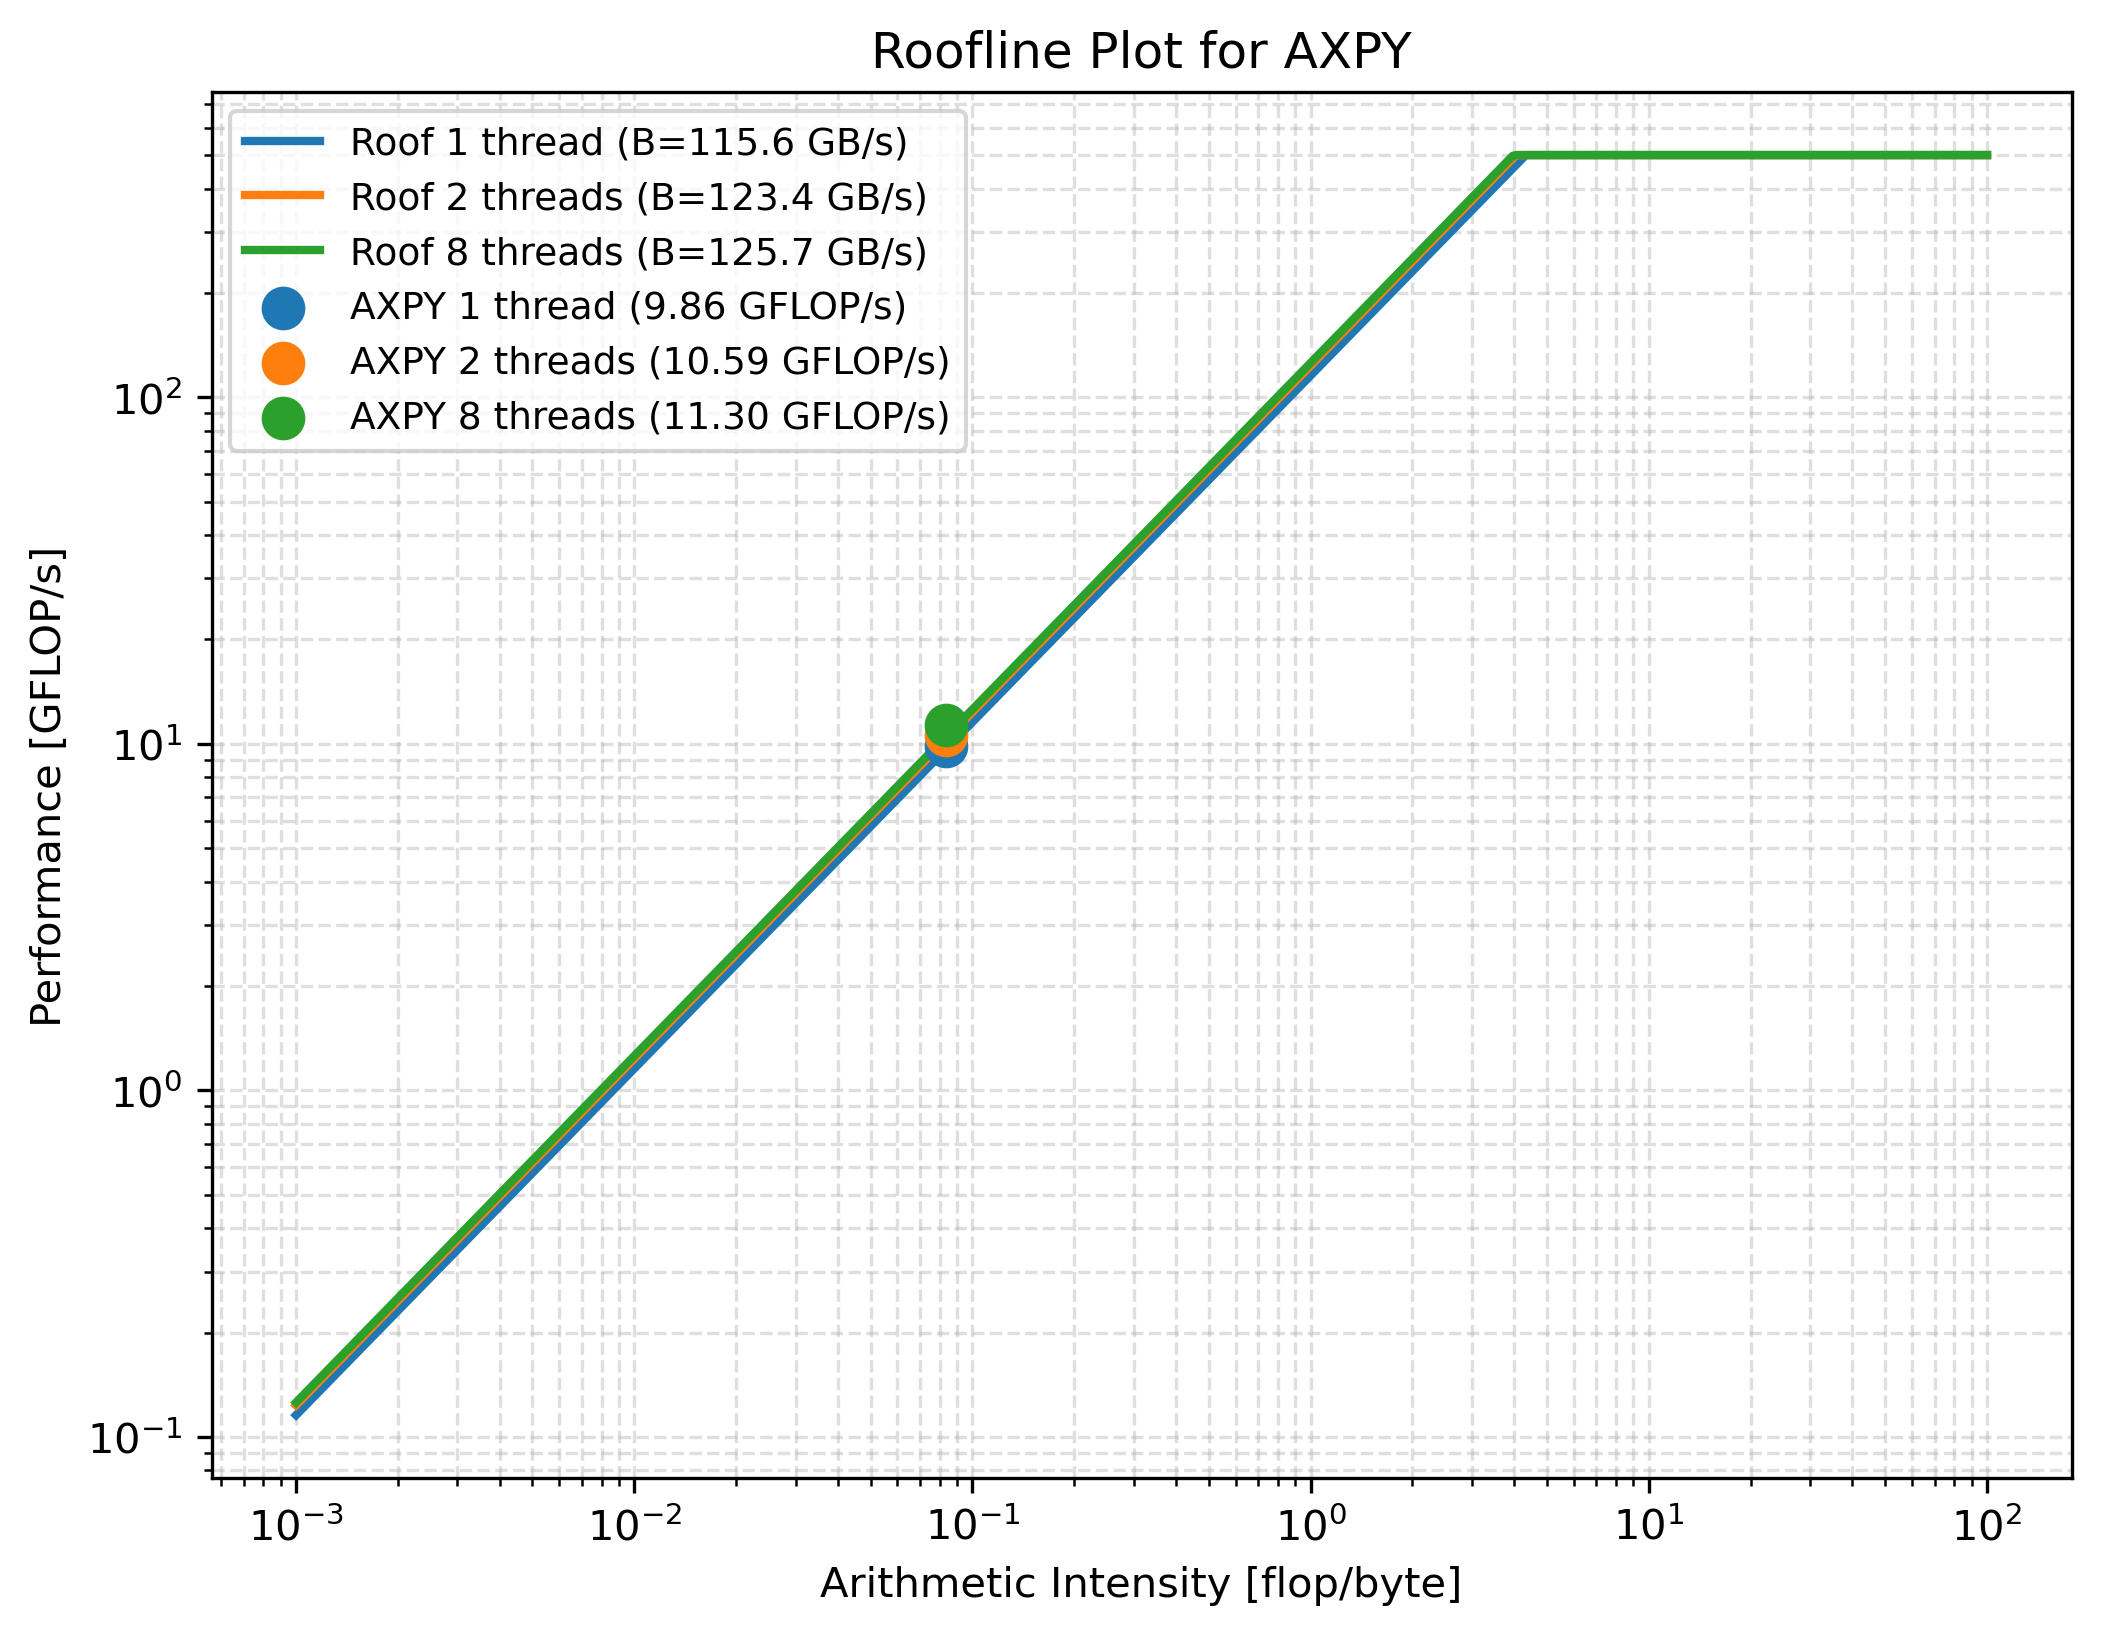
\includegraphics[width=0.6\textwidth]{roofline_plot.png}
    \caption{Roofline plots for 1 thread, 2 threads, and for 8 threads.}
    \label{fig:myfigure}
\end{figure}

Figure 1. shows the roofline analysis for the optimized AXPY implementation using 1, 2, and 8 threads. Since AXPY has a low arithmetic intensity, $I =2/24 \approx 0.0833$ flop/byte, its performance is limited by memory bandwidth rather than peak floating-point throughput. The measured points lie near the sloped bandwidth roofs, confirming that the kernel is memory-bound. The performance improves only modestly from 1 thread to 8 threads, which is consistent with the strong-scaling results and indicates that the available memory bandwidth saturates quickly.

\section{Implementing Threaded Matrix Multiplication}

\begin{enumerate}
    \item For this part, I have just modified the matmul\_blocked.cpp given in the module. We compared \texttt{\#pragma omp parallel for}, \texttt{\#pragma omp parallel for collapse(2)}, and \texttt{\#pragma omp parallel for collapse(3)} for cache-blocked matrix multiplication of size $2048 \times\,  2048$.  
    \begin{table}[h!]
\centering
 
\begin{tabular}{|c|c|c|c|c|}
\hline
\textbf{Threads} & \textbf{Time (s)} & \textbf{Speedup} & \textbf{Efficiency} & \textbf{GFLOPS} \\
\hline
1  & 4.640300 & 0.998647 & 0.998647 & 3.702319 \\
2  & 2.161789 & 2.143605 & 1.071802 & 7.947059 \\
4  & 1.298944 & 3.567530 & 0.891882 & 13.226024 \\
8  & 0.685758 & 6.757521 & 0.844690 & 25.052387 \\
16 & 0.464759 & 9.970803 & 0.623175 & 36.965095 \\
\hline
\end{tabular}
\caption{Strong scaling results for cache-blocked OpenMP matrix multiplication on NOTSx ($n=2048$, block size $=128$).}
\label{tab:blocked_strong_notsx}
\end{table}

On NOTSx, the cache-blocked OpenMP matrix multiplication performed best with plain \texttt{\#pragma omp parallel for}, which outperformed both \texttt{collapse(2)} and \texttt{collapse(3)} at 16 threads. In the strong scaling study, the implementation achieved a speedup of factor 9.97 at 16 threads, demonstrating good parallel performance.

\begin{table}[h!]
\centering
 
\begin{tabular}{|c|c|c|c|}
\hline
\textbf{Threads} & \textbf{Matrix size $n$} & \textbf{Time (s)} & \textbf{Relative to 1 thread} \\
\hline
1  & 384  & 0.015497 & 1.000000 \\
2  & 512  & 0.019252 & 1.242327 \\
4  & 640  & 0.030375 & 1.960103 \\
8  & 768  & 0.022522 & 1.453343 \\
16 & 1024 & 0.045152 & 2.913646 \\
\hline
\end{tabular}
\caption{Weak scaling results for cache-blocked OpenMP matrix multiplication on NOTSx.}
\label{tab:blocked_weak_notsx}
\end{table}

For the weak scaling study, the matrix size was chosen according to \(n \approx n_0 p^{1/3}\), so that the total computational work \(O(n^3)\) grows approximately in proportion to the number of threads and the work per thread remains roughly constant. The measured runtimes were 0.0155 s, 0.0193 s, 0.0304 s, 0.0225 s, and 0.0452 s for 1, 2, 4, 8, and 16 threads, respectively. These results indicate non-ideal weak scaling, since the runtime increases overall rather than remaining constant. The loss of weak-scaling efficiency at larger thread counts is likely caused by memory-system effects, cache contention, and parallel runtime overhead.
    \item For recursive matmul, we performed both strong and weak analyses.
    \begin{table}[h!]
\centering
 
\begin{tabular}{|c|c|c|c|c|}
\hline
\textbf{Threads} & \textbf{Time (s)} & \textbf{Speedup} & \textbf{Efficiency} & \textbf{GFLOPS} \\
\hline
1  & 7.987050 & 0.990727 & 0.990727 & 2.150965 \\
2  & 4.190492 & 1.888319 & 0.944159 & 4.099726 \\
4  &1.922237& 4.116550 &1.029137 &8.937434 \\
8  & 1.184461 &6.680663 &0.835083 &14.504375 \\
16&0.982004&8.058001&0.503625&17.494712 \\
\hline
\end{tabular}
\caption{Strong scaling results for task-based recursive matrix multiplication on NOTSx ($n=2048$, 5 trials, base case $=32$, task cutoff $=256$).}
\label{tab:recursive_task_strong}
\end{table}

\begin{table}[h!]
\centering
\begin{tabular}{|c|c|c|c|}
\hline
\textbf{Threads} & \textbf{Matrix size $n$} & \textbf{Time (s)} & \textbf{Relative to 1 thread} \\
\hline
1  & 384  & 0.034680 &1.000000 \\
2  & 484  &0.040538 &1.168927 \\
4  & 610 &0.036163 &1.042766 \\
8  & 768 & 0.045338&1.307332 \\
16 & 968 & 0.077957 &2.247911 \\
\hline
\end{tabular}
\label{tab:recursive_task_weak}
\caption{Weak scaling results for task-based recursive matrix multiplication on NOTSx.}
\end{table}
\end{enumerate}
 The task-based recursive matrix multiplication shows good strong scaling on NOTSx. The runtime decreases from 7.99 seconds at one thread to 0.98 seconds at $16$ threads, corresponding to a speedup of about a factor of 8.06. The parallel efficiency remains high at moderate thread counts, although it drops at 16 threads due to tasking overhead and memory-system limitations.

For weak scaling, the runtime remains fairly stable upto 8 threads, but increases noticeably at 16 threads. this indicates that the recursive task-based implementation exhibits reasonable weak scaling at low to moderate thread counts.

\section{Integration Implementation}

For this, I have reused the integration.cpp script provided on Canvas. In order to run this strong scaling code, just use the makefile as 

\begin{verbatim}
    $ make
    $ ./integration all 500000 8 4
\end{verbatim}

where 500000 is the number of steps, 8 is the maximum number of threads we used, and 4 is the number of times you want to repeat the calculation. 
\begin{table}[h!]
\centering
\begin{tabular}{lccc}
\hline
Implementation & Threads & Runtime (s) & Parallel Efficiency \\
\hline
Reduction & 1 & 0.000635 & 1.0000 \\
Reduction & 2 & 0.000318 & 0.9997 \\
Reduction & 4 & 0.000171 & 0.9289 \\
Reduction & 8 & 0.000094 & 0.8440 \\
\hline
Atomic & 1 & 0.004899 & 1.0000 \\
Atomic & 2 & 0.029178 & 0.0840 \\
Atomic & 4 & 0.035034 & 0.0350 \\
Atomic & 8 & 0.035398 & 0.0173 \\
\hline
\end{tabular}
\caption{Strong scaling results for the OpenMP reduction-based and atomic-based integration implementations.}
\label{tab:integration_scaling}
\end{table}

The parallel efficiency is compared with the runtime of the code with respect to the runtime using a single thread of that particular method. From Table 8., it is clear that OpenMP based reduction integration implementation exhibited excellent scalibility, achieving nearly ideal efficiency at 2 threads (99.97\%) and maintaining high efficiency at 8 threads (84.4\%). In contrast, the atomic implementation scaled very poorly, with just 8.4\% efficiency with 2 threads and eventually dropping to 1.7\% with 8 threads. The atomic implementation also became slower as the number of threads increased. The reason atomic implementation scales badly because of memory contention and synchronization cost. In contrast, the reduction implementation avoids this bottleneck by using thread-local partial sums and combining them only once at the end.
\end{document}
